\subsubsection{11.02.15 (Соревнования)}
\begin{center}
	1-ый день соревнований "Робофест-7 в Москве"
\end{center}
Сегодня был технический день, который мы посвятили общению с другими командами, отладке программ автономного периода и тренировкам.\newline

Сначала мы поговорили со всеми командами в категории FTC. Их было зарегистрировано 33, но участвовали только 32. Мы узнали возможности каждой команды в управляемом периоде, качество выполнения автономной программы (а также место старта), стратегию в игре и требования к союзнику по альянсу. Благодаря этому мы смогли получить статистические данные об уровне команд на соревнованиях и о том, с какими командами у нас получится эффективное взаимодействие. Также мы раздали каждой команде листовки, в которых содержалась краткая информация о нашей команде и наших игровых возможностях. Таким образом мы привлекли внимание к нашей команде для того, чтобы у нас было больше шансов быть выбранными в альянс в финале.\newline

Кроме того, сегодня нами были сданы на рассмотрение судей технические книги (на русском и английском языках).\newline

Внесенные доработки:
\begin{enumerate}
	\item В процессе тренировок нами было замечено, что правый угол ковша (если смотреть сзади) часто зацепляется за провод, ведущий к сервоприводу механизма опрокидывания, и не опускается до конца. Чтобы это исправить, мы срезали угол ковша и приклеили к месту среза соразмерную треугольную заплатку. После этого мы укрепили швы армированным скотчем. После того, как угол был удален, ковш перестал застревать на проводе.
	\begin{figure}[H]
		\begin{minipage}[h]{0.47\linewidth}
			\center{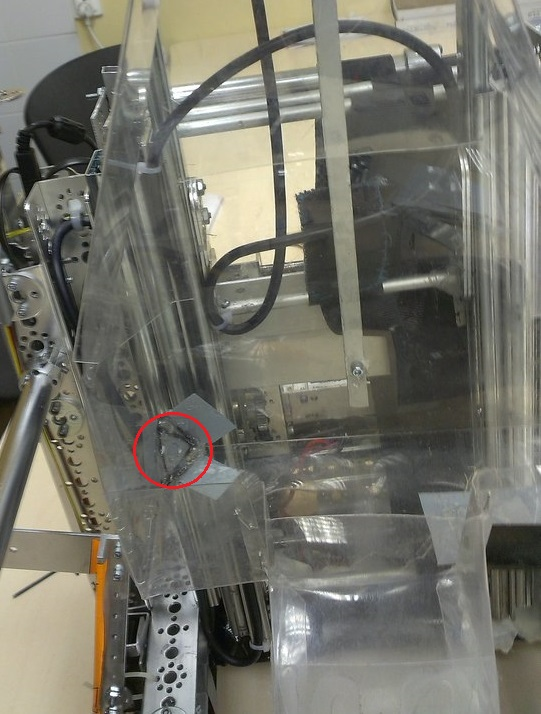
\includegraphics[scale=0.25]{days/11.02.15/images/01}}
			\caption{Срезанный угол}
		\end{minipage}
		\hfill
		\begin{minipage}[h]{0.47\linewidth}
			\center{
\includegraphics[scale=0.7]{days/11.02.15/images/02}}
			\caption{Приближенное изображение}
		\end{minipage}
	\end{figure}
	
	\item Так как почти все команды FTC лучше реализовали программу автономного периода с пандуса, чем из зоны парковки, мы решили сконцентрировать все свои силы на подготовке автономного периода из зоны парковки для того, чтобы к началу квалификационных заездов у нас была одна, но зато хорошо работающая программа автонома.
	
	\item Поскольку направляющая для мячей была закреплена только двумя болтами (по одному с каждой стороны), в моменты, когда на нее оказывалось давление (например, при соприкосновении с подвижной корзиной или про столкновении с другим роботом) она проворачивалась на винтах и отклонялась от нужного положения. Для того, чтобы это исправить, мы решили затянуть винты как можно сильнее, но через некоторое время они разбалтывались, поэтому мы установили стопор, который ограничивал люфт направляющей. Таким образом проблема была решена.
	\begin{figure}[H]
		\begin{minipage}[h]{0.2\linewidth}
			\center  
		\end{minipage}
		\begin{minipage}[h]{0.6\linewidth}
			\center{
\includegraphics[scale=0.2]{days/11.02.15/images/03}}
			\caption{Ограничитель}
		\end{minipage}
	\end{figure}
	
\end{enumerate}
\fillpage
